





\section{Frequency analysis}
\label{sec:analysis}
\subsection{Car engine}

\begin{figure}
	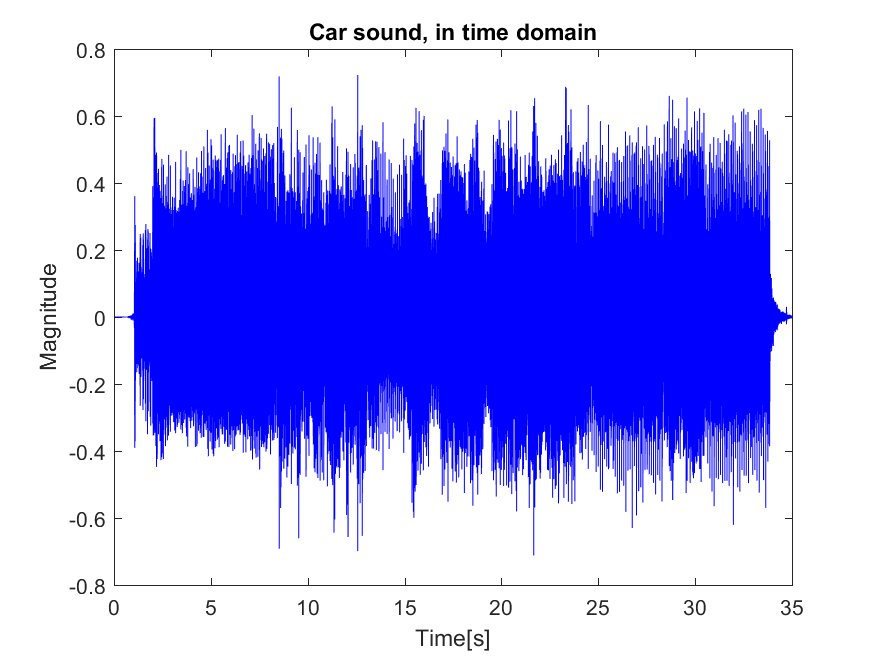
\includegraphics[width=\textwidth]{code/Car_figure1.png}
	\caption{kage}
	\label{fig:Car_figure1:1}
\end{figure}

\subsubsection{DFT}
\begin{figure}
	\centering
	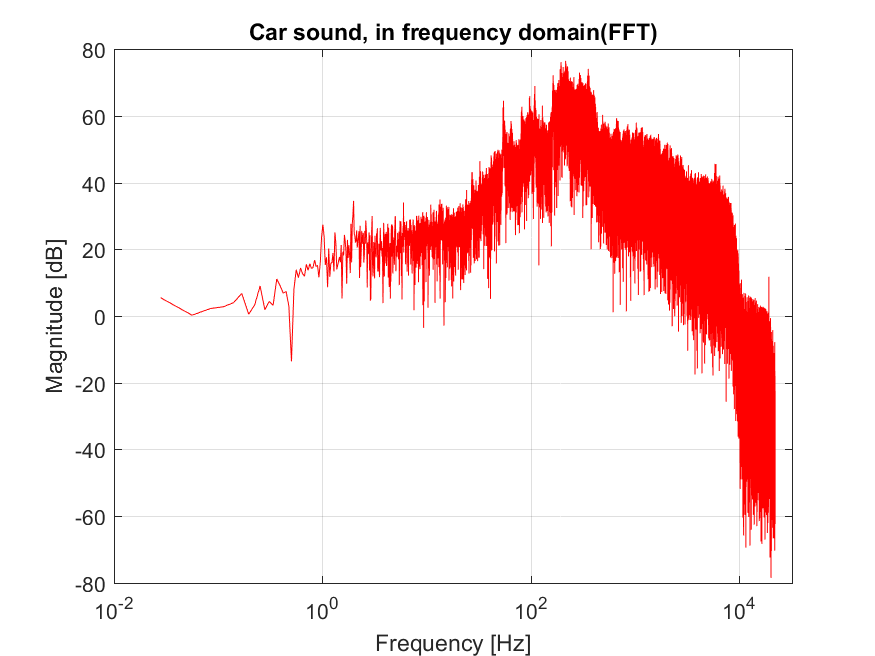
\includegraphics[width=\textwidth]{code/Car_figure2.png}
	\caption{}
	\label{fig:Car_figure2:2}
\end{figure}




\subsubsection{Analysis}



\subsubsection{Conclusion}

\subsection{Noise from a windmill}
\subsubsection{DFT}

\subsubsection{Analysis}

\subsubsection{Conclusion}

\subsection{EKG}
\subsubsection{DFT}

\subsubsection{Analysis}

\subsubsection{Conclusion}

\subsection{Breaking wine glass}
\subsubsection{DFT}

\subsubsection{Analysis}

\subsubsection{Conclusion}

\subsection{Music}
\subsubsection{DFT}

\subsubsection{Analysis}

\paragraph{Genre 1}

\paragraph{Genre 2}

\paragraph{Genre 3}

\paragraph{Genre 4}

\subsubsection{Conclusion}

\section{Further analysis of signals}
\label{sec:analysisOfSignals}
Eksperimenter med udglatning, zero-padding og windowing 

\section{Energy} 
table \ref{tab:Energy} shows the energies in signals before and after the fourier transform. And it clearly shows that there is no loss of energy and a Fourier transform.
but when smoothing and windowing is applied there is a potential loss of energy. While zero pad doesn't add or remove any energy from the signal
\begin{table}[]
\centering
\begin{tabularx}{\textwidth}{Xllll}
windmill                      &                  &           &           &           \\
time domain                   & frequency domain & smoot     & zero pad  & Windowing \\
4,141E+04                     & 4,141E+04        & 7,100E+02 & 4,141E+04 & 1,793E+04 \\
                              &                  &           &           &           \\
car sound                     &                  &           &           &           \\
time domain                   & frequency domain & smoot     & zero pad  & Windowing \\
3,07E+04                      & 3,07E+04         & 6,86E+02  & 3,07E+04  & 1,34E+04  \\
                              &                  &           &           &           \\
                              &                  &           &           &           \\
Cheerleader                   &                  &           &           &           \\
time domain                   & frequency domain & smoot     & zero pad  & Windowing \\
1,34E+05                      & 1,34E+05         & 1,29E+03  & 1,34E+05  & 7,39E+04  \\
                              &                  &           &           &           \\
Roundtable Rival              &                  &           &           &           \\
time domain                   & frequency domain & smoot     & zero pad  & Windowing \\
2,98E+05                      & 2,98E+05         & 1,70E+03  & 2,98E+05  & 1,28E+05  \\
                              &                  &           &           &           \\
Michael Jackson - Billie Jean &                  &           &           &           \\
time domain                   & frequency domain & smoot     & zero pad  & Windowing \\
1,627E+05                     & 1,627E+05        & 1,727E+03 & 1,627E+05 & 6,862E+04 \\
                              &                  &           &           &           \\
Let-It-Go Violin              &                  &           &           &           \\
time domain                   & frequency domain & smoot     & zero pad  & Windowing \\
2,24E+04                      & 2,24E+04         & 896,4634  & 2,24E+04  & 1,09E+04  \\
                              &                  &           &           &           \\
crystalglass                  &                  &           &           &           \\
time domain                   & frequency domain & smoot     & zero pad  & Windowing \\
115,23                        & 115,23           & 154,83    & 115,23    & 2,65      \\
                              &                  &           &           &           \\
heartmonitor-ekg              &                  &           &           &           \\
time domain                   & frequency domain & smoot     & zero pad  & Windowing \\
2,05E+04                      & 2,05E+04         & 626       & 2,05E+04  & 7,29E+03 
\end{tabularx}

\caption{energy in different signals after, different analysis methods }
\label{tab:Energy}
\end{table}

\section{Discussion}

Skalering --> Vi kan ikke bruge frekvenser højere end nyquits frekvens ?
Korrekte frekvensbins?

\section{Conclusion}